% Système mobile d’imagerie interventionnelle Discovery IGS 730

\section{Présentation du système}
\subsection{Mise en situation}
Développé dans le cadre d’un projet ambitieux associant des industriels (GE Healthcare, BA Systèmes et C\&K), deux laboratoires de recherche (CEA-LIST et IRCCYN) et un centre de recherche
préclinique (laboratoire CR2i INRA AP-HP), le Discovery IGS 730 (figure 1) est le premier système
mobile d’imagerie interventionnelle. Embarquant un ensemble de logiciels de traitement d’images
pour les applications vasculaires, l’oncologie et la cardiologie (figure 2) et permettant un accès complet au patient, il guide les gestes de l’équipe médicale tout au long de l’intervention chirurgicale.

\begin{figure}[!h]
\centering
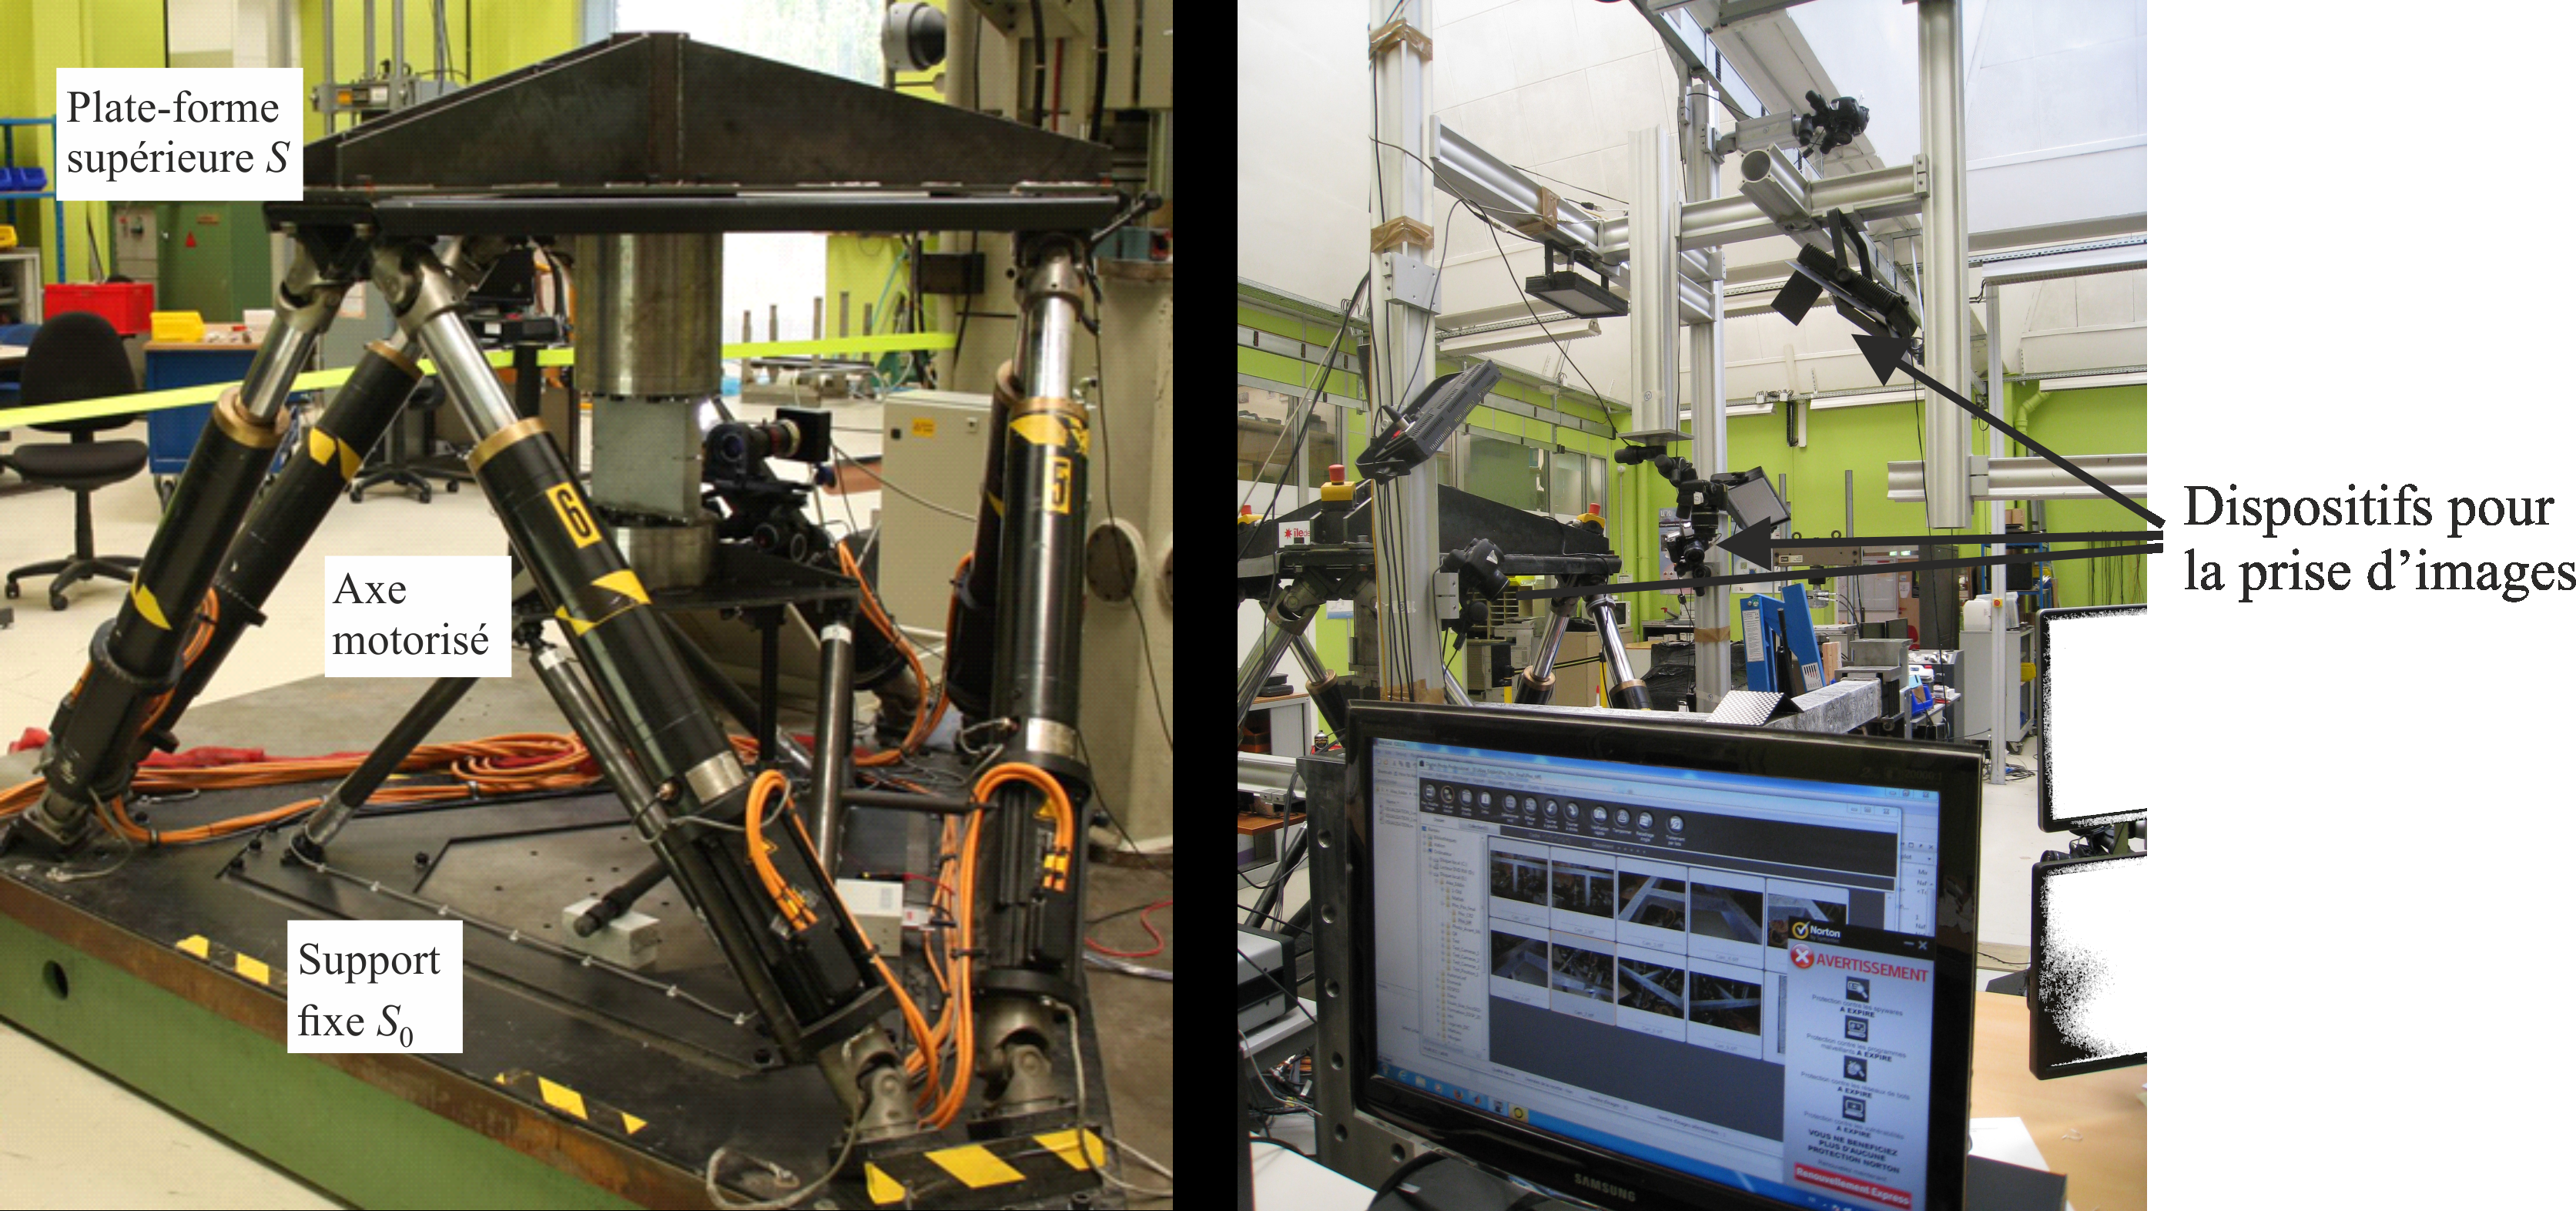
\includegraphics[width=\linewidth]{fig_01}
\caption{\label{fig:01}  Système d’imagerie robotisé Discovery IGS 730 en situation de travail (photo de gauche) et en mode parking (photo de droite).}
\end{figure}


\begin{figure}[!h]
\centering
	\begin{subfigure}[b]{0.3\textwidth}
	\centering
	\includegraphics[height=4cm]{fig_02_a}
	\caption{\label{fig:02a} Système vasculaire du poumon.}	
	\end{subfigure}
	\begin{subfigure}[b]{0.3\textwidth}
	\centering
	\includegraphics[height=4cm]{fig_02_b}
	\caption{\label{fig:02b} Système vasculaire général.}
	\end{subfigure}


\caption{\label{fig:02}  Images 3D obtenues avec le système d’imagerie du Discovery IGS 730.}
\end{figure}

Le Discovery IGS 730 révolutionne le domaine de l’imagerie interventionnelle. Contrairement aux
systèmes d’angiographie traditionnels, il n’est ni fixé au sol, ni suspendu au plafond, mais dispose
d’une base motorisée guidée par laser qui transporte l’arceau d’imagerie. Cette innovation technologique offre une mobilité totale au système qui peut, par exemple, rejoindre de manière autonome
une position « parking » prédéfinie afin de laisser tout le champ disponible à l’équipe médicale pour
s’occuper du patient. Ce gain de mobilité permet également une intégration aisée en milieu clinique,
un accès facilité au patient et des possibilités de positionnement illimitées.


\subsection{Analyse système partielle}
La figure 3 présente un extrait du cahier des charges du système d’imagerie dans la phase de vie
d’utilisation. La figure 4 présente son diagramme de définition des blocs.


\begin{figure}[!h]
\centering
\includegraphics[width=\linewidth]{fig_03}
\caption{\label{fig:03}  Diagramme d’exigences partiel du Discovery IGS 730.}
\end{figure}


\begin{figure}[!h]
\centering
\includegraphics[width=\linewidth]{fig_04}
\caption{\label{fig:04}  Diagramme de définition de blocs du Discovery IGS 730.}
\end{figure}

Le système Discovery IGS 730 est constitué principalement (figure 4, page 3 et figure 5) :
\begin{itemize}
\item d’une base motorisée, aussi appelée AGV (pour Automated Guided Vehicle, soit véhicule à
guidage automatique) ;
\item d’une perche et d’un support de câbles ;
\item du sous-système d’imagerie supporté par un bras en « C » ou arceau. Le système d’imagerie
est lié à la base motorisée par l’intermédiaire de deux liaisons pivot. Un point caractéristique
appelé « isocentre » (point $I_C$) est rattaché au sous-système d’imagerie. Il est défini comme
l’intersection de l’axe optique et de l’axe de la liaison pivot AGV/système pivot.
\end{itemize}

\begin{figure}[!h]
\centering
\includegraphics[width=.6\linewidth]{fig_05}
\caption{\label{fig:05}  Composants du Discovery IGS 730.}
\end{figure}

La base motorisée AGV (figure 6) est constituée :
\begin{itemize}
\item d’une structure support, ou châssis, composée du bras vertical et du cadre Y ;
\item de deux sous-ensembles roue motrice et motorisation associée (un motoréducteur d’orientation et un motoréducteur de propulsion pour chaque roue) ;
\item de deux doubles roues « folles » non motorisées.
\end{itemize}

\begin{figure}[!h]
\centering
\includegraphics[width=\linewidth]{fig_06}
\caption{\label{fig:06} Éléments du sous-système AGV, carter et sous-système d’imagerie enlevés.}
\end{figure}

\subsection{Problème posé}
La mobilité totale apportée au Discovery IGS 730, véritable innovation technologique dans le domaine de l’imagerie interventionnelle, a conduit les ingénieurs responsables du développement à travailler sur des problématiques spécifiques liées :
\begin{itemize}
\item à la maîtrise du positionnement du sous-système d’imagerie par rapport au patient ;
\item à la sécurité du patient et de l’équipe médicale au cours des déplacements du système dans la
salle d’intervention.
\end{itemize}
\begin{obj}
L’objectif de cette étude est de vérifier certaines performances du système afin de valider partiellement le respect des exigences liées au positionnement de l’AGV et par suite, du sous-système
d’imagerie (Id. 1.1) et à la sécurité des personnes au cours des déplacements (Id. 1.2).
\end{obj}


\subsection{Démarche}

Le respect des exigences relatives au positionnement du sous-système d’imagerie (Id. 1.1), objet de
la partie 2, est abordé à travers les points suivants :
\begin{itemize}
\item étude géométrique et cinématique de l’AGV afin d’estimer la précision requise au niveau de
l’orientation des roues motrices (Id. 1.1.2) ;
\item prévision des performances de la commande associée au mouvement de translation de la base
motorisée (Id. 1.1.3) ;
\item étude de la stratégie de localisation de l’AGV et développement d’algorithmes d’estimation
de sa position (Id. 1.1.1).
\end{itemize}
Le respect des exigences relatives à la sécurité des personnes (Id. 1.2) fait l’objet de la partie 3 consacrée à la prévision du comportement dynamique du système lors d’un freinage d’urgence intervenant
au cours d’une manœuvre de translation (Id. 1.2.1.1).

\section{Validation des exigences relatives au positionnement du sous-système d’imagerie}
\subsection{Modélisation géométrique et cinématique de l’AGV}
\begin{obj}
Vérifier que l’exigence « Précision de positionnement de l’axe de rotation » (Id. 1.1.2.1) peut
être satisfaite.
\end{obj}


Au cours d’une intervention médicale ou de certains examens d’imagerie, l’ensemble du système
est amené à pivoter autour du patient suivant un axe vertical. Afin de ne pas perturber le processus
d’acquisition, la position de l’isocentre $I_C$ par rapport au patient ne doit pas varier durant la manœuvre
(figure 5). Il est donc nécessaire de maîtriser, par le biais de l’orientation des roues motrices, le
positionnement de l’axe de pivotement du système, afin que celui-ci passe par l’isocentre $I_C$.

\subsection*{Paramétrage et hypothèses}

Le modèle géométrique retenu et le paramétrage associé sont donnés sur la figure 7, page 6.

Les repères et angles suivants sont introduits pour l’étude :
\begin{itemize}
\item $\rep{0}$ est un repère attaché à la salle d’intervention. Il a pour origine l’isocentre $I_C$ (supposé fixe
dans la salle) et pour base $\base{x_{0}}{y_{0}}{z_{0}}$ tel que le vecteur $z_{0}$ soit vertical ascendant ;
\item $\rep{C} \repere{I_C}{x_{C}}{y_{C}}{z_{0}}$, repère associé au cadre Y, avec $\psi = \angl{x_{0}}{x_{C}}= \angl{y_{0}}{y_{C}}$ l’angle associé à la
rotation du cadre Y autour de l’axe vertical $\axe{I_C}{z_{0}}$ passant par l’isocentre ;
\item $\rep{P}\repere{A}{x_{P}}{y_{P}}{z_{0}}$ repère associé à la liaison pivot d’axe $\axe{A}{z_{0}}$ de la roue motrice droite avec le
cadre Y, avec $\beta = \angl{x_{C}}{x_{P}}= \angl{y_{C}}{y_{P}}$ l’angle associé à l’orientation de la roue motrice droite
($R_D$) par rapport au cadre Y ;
\item $\rep{R}\repere{A}{x_{R_D}}{y_{P}}{z_{R_D}}$, repère associé à la roue motrice droite ($R_D$), avec $\theta_D = \angl{x_{P}}{x_{R_D}}= \angl{z_{0}}{z_{R_D}}$ 
l’angle associé à la rotation de la roue motrice droite ($R_D$) autour de l’axe $\axe{A}{x_{R_D}}$.
\end{itemize}

L’AGV est animé d’un mouvement de rotation autour de l’axe $\axe{I}{z_0}$; sa géométrie est considérée
comme symétrique par rapport à l’axe $\axe{I}{y_c}$.
Les dimensions utiles ont pour valeurs : $a = \SI{1 440}{mm}$, $e = \SI{800}{mm}$, $r = AI_D = \SI{115}{mm}$.

\begin{figure}[!h]
\centering
\includegraphics[width=\linewidth]{fig_07}
\caption{\label{fig:07} Modèle retenu pour l’étude géométrique (à gauche, vue du demi-système).}
\end{figure}

Les hypothèses suivantes sont adoptées :
\begin{itemize}
\item les contacts roue-sol sont modélisés par des contacts ponctuels (point $I_D$ pour la roue motrice
droite) et les roues motrices roulent sans glisser sur le sol,
\item les taux de rotation des roues motrices droite $\thetap_D$ et gauche $\thetap_G$ sont égaux.
On notera que l’angle $\beta$ est négatif sur la figure 7.
\end{itemize}

\subsection*{Étude du positionnement angulaire des roues motrices}

%Q1.
\question{En exploitant la condition de roulement sans glissement au point $I_D$, déterminer l’expression
du vecteur vitesse $\vectv{A}{\text{cadre}}{\rep{0}}$ dans la base du repère $\rep{P}$ en fonction de $\thetap_D$ et du rayon de roue $r$.}

La figure 7 montre un décalage $\Delta y$ entre l’axe de rotation du cadre $\axe{I}{z_0}$ et l’axe vertical passant par 
l’isocentre $\axe{I_C}{z_0}$. Lorsque l’isocentre $I_C$ est situé sur l’axe de rotation du mouvement du cadre par
rapport à $\rep{0}$ (soit $\Delta y = 0$), la relation suivante est vérifiée :  $\vect{I_C A}\cdot \vectv{A}{\text{cadre}}{\rep{0}}=\vect{0}$.

%Q2. 
\question{En exploitant cette dernière relation, déterminer en fonction des paramètres géométriques
utiles, l’expression de l’angle $\beta$ correspondant. Calculer sa valeur numérique en degrés.}

Le constructeur du groupe motoréducteur dédié à l’orientation de la roue motrice garantit une précision 
angulaire $\Delta \beta = \pm 10^{-3}$ degrés pour l’angle d’orientation $\beta$.

%Q3. 
\question{En prenant comme référence la configuration pour laquelle l’isocentre $I_C$ est situé sur l’axe
de la rotation, déterminer la valeur de $\Delta y$ associée à une erreur angulaire 
$\Delta \beta = \pm 10^{-3} $ degrés. Conclure quant au respect de l’exigence (Id. 1.1.2.1).}


\subsection{Prévision des performances « l’asservissement en vitesse du mouvement de translation de
l’AGV »}

\begin{obj}
Vérifier que l’exigence d’asservissement en vitesse du mouvement de translation de la base motorisée AGV (Id. 1.1.3) et ses sous-exigences sont respectées.
\end{obj}

Les déplacements de la base motorisée AGV sont contrôlés de la manière suivante : au niveau de
chacun des 2 moteurs, des boucles de vitesse et de position assurent l’asservissement en vitesse et
position du système. Nous ne nous intéresserons dans le sujet qu’à la boucle de vitesse. L’objectif de
cette partie est de déterminer les paramètres de réglage de chacune des boucles d’asservissement en
vitesse lors d’un mouvement de translation de l’AGV par rapport au sol.

\subsection*{Étude préliminaire : moteurs brushless de propulsion}

\subsection*{Hypothèses et modélisations}
\begin{itemize}
\item l’AGV se déplace en ligne droite (consigne de vitesse $v_c(t)$, les roues étant dans la même
direction que l’axe de symétrie de l’AGV) ;
\item les roues motrices roulent sans glisser sur le sol ;
\item la charge extérieure est supposée équi-répartie sur chacun des deux moteurs. Ainsi, pour une
vitesse $v(t)$ de la plateforme, les deux moteurs de propulsion tournent à la même vitesse angulaire $\omega_m(t)$, sont alimentés par une même tension de commande $u(t)$ et fournissent un même
couple moteur $C_m(t)$ ;
\item les perturbations sont réparties sur chacun des axes des deux moteurs et sont modélisées par
un même couple de perturbation équivalent appliqué sur chacun des axes moteurs $C_r(t)$ ;
\item les caractéristiques inertielles de la plateforme sont représentées au niveau de chaque axe
moteur par un moment d’inertie équivalent $\indice{J}{eq}$ ;
\item le comportement individuel d’un des deux moteurs brushless peut être approché par celui d’un
moteur à courant continu avec les équations électromécaniques suivantes :
$u(t)=E(t)+Ri(t)+L\dfrac{\dd i(t)}{\dd t}$, $C_m(t)=K_c i(t)$, $e(t)=K_e \omega_m(t)$ et $C_m(t)-C_r(t)=\indice{J}{eq} \dfrac{\dd \omega_m(t)}{\dd t}  $. 
\end{itemize}

\begin{table}[!h]
\centering
\begin{tabular}{lll}
\hline
\textbf{Symbole} & \textbf{Désignation} & \textbf{Valeurs, unités} \\
\hline
$u(t)$ 		& Tension d’alimentation du moteur 		& [V] \\
$e(t)$ 		& Tension contre-électromotrice dans un moteur 	&[V] \\
$i(t)$	 	& Intensité du courant dans un moteur 		& [A] \\
$v(t)$ 		& Vitesse de translation du système 		& [m/s] \\
$\omega_m(t)$	& Vitesse angulaire de chacun des deux moteurs	& [rad/s]\\
$C_m(t)$ 	& Couple moteur appliqué par chacun des deux moteurs & [N.m]\\
$C_r(t)$	& Couple de perturbation équivalent appliqué à chacun des deux axes moteurs & [N.m] \\
$R$ 		& Résistance de l’induit d’un moteur 		& \SI{0,07}{\Omega} \\
$L$ 		& Inductance de l’induit d’un moteur 		& \SI{0,15}{mH} \\
$K_e$ 		& Constante de vitesse d’un moteur 		& \SI{0,113}{V/(rad/s)}\\
$K_c$ 		& Constante de couple d’un moteur 		& \SI{0,113}{N.m/A}\\
$\indice{J}{eq}$& Inertie équivalente de la moitié du système ramenée sur l’axe d’un moteur 
								& \SI{5,3e-3}{kg.m^2}\\\hline
\end{tabular}
\end{table}

\subsection*{Fonction de transfert d’un moteur de propulsion}

On note $\Omega_m(p)$, $U(p)$, $E(p)$, $I(p)$, $C_m(p)$ et $C_r(p)$ les transformées de Laplace respectives de $\omega_m(t)$,
$u(t)$, $e(t)$, $i(t)$, $C_m(t)$ et $C_r(t)$.

\question{Déterminer sur la copie les transformées de Laplace des équations (1) à (4) du moteur définies en considérant des conditions initiales nulles. Compléter le schéma-bloc du document
réponse DR1 par les transmittances manquantes.}

%Q5. 
\question{Déterminer les expressions littérales des fonctions de transfert du moteur en poursuite
$H_1(p) =\left.\dfrac{\Omega_m(p)}{U(p)}\right|_{C_r(p)=0}$ (sans perturbation) et en régulation 
$H_2(p) =\left.\dfrac{\Omega_m(p)}{C_r(p)}\right|_{U(p)=0}$, sous forme
canonique. Par application du principe de superposition, en déduire l’expression de $\Omega_m(p)$ en
fonction de $U(p)$ et de $C_r(p)$.}

Le système est étudié en l’absence de perturbation, $C_r(t) = 0$.

%Q6. 
\question{Réaliser l’application numérique de la fonction de transfert du moteur $\dfrac{\Omega_m(p)}{U(p)}$ et mettre le résultat sous la forme : $\dfrac{K}{\left(1+\tau_1 p \right)\left(1+\tau_2 p \right)}$
.}



\subsection*{Étude de l’asservissement en vitesse de la base motorisée AGV}

Pour une consigne de vitesse $v_c(t)$ [m/s], les microcontrôleurs de pilotage génèrent une tension de
consigne de rotation à appliquer à chaque moteur $u_c(t)$ [V]. Un traitement numérique de la vitesse
relevée sur l’axe de chaque moteur fournit une tension mesurée $u_m(t)$ [V], image de la vitesse de
rotation du moteur $\omega_m(t)$. Un correcteur (défini par la suite) adapte le signal écart entre la tension de
consigne et la tension mesurée, ce qui permet après correction et amplification, de définir la tension
d’alimentation $u(t)$ à appliquer aux moteurs.

\begin{figure}[!h]
\centering
\includegraphics[width=\linewidth]{fig_08}
\caption{\label{fig:08}  Schéma-bloc fonctionnel de l’asservissement en vitesse d’un des deux moteurs.}
\end{figure}

\begin{table}[!h]
\centering
\begin{tabular}{ll}
\hline
\textbf{Blocs} & \textbf{Fonctions de transfert} \\
\hline
Convertisseur 		& $\indice{K}{conv}$  (à déterminer)\\
Correcteur		& $C(p)$ (réglé par la suite) \\
Amplificateur		& $K_A = 7,9$ sans unité \\
Traitement numérique de la vitesse 	& $\indice{K}{Vit} = \SI{1,3e-3}{V/(rad/s)}$ \\
Réduction et roue 	& $K_R$ (à déterminer) \\
\hline
\end{tabular}
\end{table}

Indépendamment des résultats trouvés précédemment, la fonction de transfert du moteur brushless
sera prise égale à : 
$H_m(p)=\dfrac{K}{\left(1+\tau_1 p \right)\left(1+\tau_2 p \right)}$ avec $K_m = 8,85$, 
$\tau_1 = \SI{0,027}{s}$ et $\tau_2 = \SI{0,0023}{s}$.



Le moteur est suivi d’un réducteur à deux étages : le premier avec un rapport de réduction 
$k_1 = \dfrac{1}{4}$ et le second avec un rapport de réduction $k_2 = \dfrac{1}{28,9}$.
Le rayon $r$ des roues motrices est de \SI{115}{mm}.

%Q7. 
\question{Déterminer les valeurs numériques et unités SI des gains $K_R$ (ensemble réducteur et roue) et
$\indice{K}{conv}$ (convertisseur) en sachant que lorsque la vitesse réelle de l’AGV $v(t)$ est égale à la vitesse de consigne $v_c(t)$, l’écart $\varepsilon(t)$ doit être nul.} 

%Q8. 
\question{Compléter le schéma-bloc sur le document réponse DR2 en y faisant figurer les fonctions de
transfert sous forme littérale dans le domaine de Laplace avec des conditions initiales nulles,
ainsi que les signes des sommateurs.}

\subsection*{Étude du système non corrigé : $C(p) = 1$}

%Q9. 
\question{Déterminer, en fonction notamment de $K_m$, $K_R$, $\indice{K}{vit}$, $\tau_1$ et $\tau_2$, l’expression de la fonction
de transfert de la boucle de vitesse sous la forme canonique d’un système du second ordre
$H(p) = \dfrac{V(p)}{V_c(p)} = \dfrac{K}{1+\dfrac{2\xi}{\omega_0}p+\dfrac{p^2}{\omega_0^2}}$. Donner les expressions littérales et numériques de $K$, $\xi$ et
$\omega_0$.}

%Q10. 
\question{Justifier que l’accélération maximum peut être approchée par $\indice{a}{max} = \dfrac{\indice{V}{max}}{t_{5\%}}$.}
%Q11. 
\question{À l’aide de l’abaque du document réponse DR3, déterminer le temps de réponse à 5 \% de la
boucle de vitesse (faire apparaître les tracés sur le document réponse). Ce temps de réponse est-il satisfaisant vis-à-vis de l’exigence Id. 1.1.3.1.1 ? Sinon, comment satisfaire cette exigence ?}

%Q12. 
\question{Déterminer l’erreur en régime permanent de la boucle de vitesse pour une entrée en échelon.
Permet-elle de satisfaire l’exigence Id. 1.1.3.2.1 ? Sinon, comment satisfaire cette exigence ?}

\subsection*{Étude du système corrigé : $C(p) = K_p\left( 1+\dfrac{1}{T_i p}\right)$.}
%Q13. 
\question{Déterminer, en fonction notamment de $K_m$, $K_R$, $\indice{K}{vit}$, $\tau_1$ et $\tau_2$, l’expression de la fonction de transfert en boucle ouverte, sous la forme canonique suivante : 
$\indice{H}{BO}(p) = \indice{K}{BO}\dfrac{Tip + 1}{p(1 + \tau_1 p)(1 + \tau_2 p)}$.
Donner l’expression littérale de $\indice{K}{BO}$.}
%Q14. 
\question{On choisit $T_i$ de façon à compenser le << mode le plus lent >>. Donner la valeur de $T_i$.}

L’exigence de stabilité Id. 1.1.3.3.1 impose une marge de phase de 45\degres.

Indépendamment de la réponse à la question précédente, on prendra $\indice{K}{BO} = 37K_p$.

%Q15. 
\question{Ce correcteur permet-il de répondre à l’exigence de précision ? Tracer les asymptotes et les
courbes réelles avec $K_p = 1$ dans le plan de Bode du document réponse DR4. Déterminer le
gain $K_p$ du correcteur permettant de satisfaire l’exigence de stabilité en étant le plus rapide (on
s’intéressera à la bande passante à \SI{0}{dB}).}

La figure du document réponse DR5 présente sur un même graphe les réponses à une consigne en
échelon d’amplitude \SI{0,3}{m/s} obtenues par simulation pour différentes valeurs de $K_p$.

%Q16. 
\question{Choisir le gain $K_p$, parmi les trois valeurs proposées, satisfaisant l’exigence de stabilité et de
rapidité (notamment l’accélération qui ne doit pas dépasser \SI{0,8}{m/s^2}. Appuyez votre réponse
par des tracés sur le document réponse DR5.}

\subsection*{SYNTHÈSE}
%Q17. 
\question{Les courbes du document réponse DR6 représentent la réponse réelle relevée sur la base
motorisée AGV et le résultat obtenu par simulation numérique pour une entrée en échelon
d’amplitude \SI{0,3}{m/s}. Comparer quantitativement les résultats au cahier des charges et conclure
sur les écarts.}



\subsection*{ Localisation de l’AGV : estimation de la position}
\begin{obj}
Mettre en place une stratégie pour répondre à l’exigence « Localiser la base motorisée AGV
dans la salle d’intervention » (Id. 1.1.1) et développer les algorithmes de traitement numérique
visant à estimer la position de l’AGV.
\end{obj}


Les questions d’informatique peuvent être traitées en langage Python ou langage Scilab. Il est
demandé au candidat de bien préciser sur sa copie le choix du langage et de rédiger l’ensemble
de ses réponses dans ce langage. L’annexe page 16 rappelle les principales commandes utiles à
la manipulation des vecteurs et matrices.
Dans tout le sujet, il sera supposé que les modules et bibliothèques sont déjà importés dans le
programme.

\subsection*{Localisation par odométrie}
La gestion des déplacements du système au sein de
la salle d’intervention (figure 9) nécessite de déterminer la position de la plateforme mobile, repérée
par le vecteur position $p$, tel que
$p 
= 
\begin{bmatrix}
x(t)\\
y(t)\\
\theta(t)
\end{bmatrix}
$
où $x(t)$, $y(t)$ et $\theta(t)$ sont les paramètres de position
définis dans le repère global $\left(O, \vect{x_0}, \vect{y_0}\right)$ associé à la
salle d’intervention.

\begin{figure}[!h]
\centering
\includegraphics[width=.7\linewidth]{fig_09}
\caption{\label{fig:09}  Paramétrage.}
\end{figure}

Une première stratégie de localisation a conduit à estimer les paramètres de position par odométrie :
partant d’une position initiale connue, la position est actualisée au cours du mouvement en estimant le
déplacement global du système à partir des mesures des déplacements angulaires des roues motrices
délivrées par les codeurs de roue. Pour cette étude, l’orientation des roues motrices par rapport à la
plateforme mobile suivant $\vect{z_0}$ est supposée fixée, dans la configuration de la figure 9.

Soient $\Delta \theta_D$ et $\Delta \theta_G$ les déplacements angulaires des roues motrices droite et gauche et $\Delta \bm{p}$ le vecteur
associé au déplacement global de la plateforme entre les instants $t$ et $(t + \Delta t)$, $\Delta t$ étant la durée d’une
période d’échantillonnage séparant deux mesures. Il est admis ici que les composantes $\left(\Delta x, \Delta y, \Delta \theta \right)$
du déplacement global $\Delta \bm{p}$ peuvent être estimées à partir de $\Delta \theta_D$ et $\Delta \theta_G$ selon :
$$
\left\{
\begin{array}{l}
\Delta x = r \dfrac{\Delta \theta_D+\Delta \theta_G}{2} \cos \left(\theta(t) + r \dfrac{\Delta \theta_D-\Delta \theta_G}{2e}\right) \\
\Delta y = r \dfrac{\Delta \theta_D+\Delta \theta_G}{2} \sin \left(\theta(t) + r \dfrac{\Delta \theta_D-\Delta \theta_G}{2e}\right) \\
\Delta \theta = r \dfrac{\Delta \theta_D-\Delta \theta_G}{e}
\end{array}
\right.
$$

où $r$ est le rayon d’une roue motrice et e la distance entre les deux roues motrices.
Le vecteur position à l’instant $(t + \Delta t)$ noté $\bm{p'}$ est alors calculé suivant : $\bm{p'}=\bm{p}+\Delta \bm{p}$.
Le traitement numérique repose sur une fonction \lstinline{position_odometrie(delta_d,delta_g, p0)}
qui prend en arguments :
\begin{itemize}
\item \lstinline{delta_d} et \lstinline{delta_g}, déplacements angulaires des roues droite ($\Delta \theta_D$) et gauche ($\Delta \theta_D$) ;
\item \lstinline{p0}, tableau de dimension 3 associé à la position à l’instant $t$ (vecteur $\bm{p}$).
\end{itemize}
La fonction renvoie le tableau \lstinline{p1} de dimension 3 associé à la position à l’instant $(t + \Delta t)$ (vecteur $\bm{p'}$). Les paramètres géométriques $r$ et $e$ sont déclarés comme variables globales dans le programme principal.

%Q18. 
\question{Écrire la fonction \lstinline{position_odometrie(delta_d,delta_g,p0)} renvoyant le tableau \lstinline{p1}.}


\subsection*{Modèle d’évolution de l’incertitude associée à l’estimation de la position}
Une approche statistique permet de modéliser l’évolution de l’incertitude sur l’estimation de la position par odométrie au cours du déplacement de l’AGV. En considérant les estimations $x$, $y$ et $\theta$ comme
des variables aléatoires continues et sous certaines hypothèses non détaillées ici, l’incertitude associée à l’estimation de la position $\bm{p'}$ peut être quantifiée par un ensemble de paramètres associés aux
variables aléatoires telles que la variance et la covariance, constituant la matrice $\Sigma_{p'}$ :
$$
\Sigma_{p'}
=
\begin{bmatrix}
\sigma_x^2 	& \sigma_{xy} 	& \sigma_{x\theta} \\
\sigma_{yx} 	& \sigma_y^2 	& \sigma_{y\theta} \\
\sigma_{zx} 	& \sigma_{zy} 	& \sigma_{\theta}^2
\end{bmatrix}
.$$

Pour le calcul de ses termes, celle-ci est décomposée suivant : 
$\Sigma_{p'} = \Sigma_1 + \Sigma_2$
où :
\begin{itemize}
\item $\Sigma_1$ est une matrice associée aux incertitudes sur l’estimation du déplacement $\Delta \bm{p} $ entre $t$ et $t+\Delta t$ à partir des mesures codeurs,
\item $\Sigma_2$ est une matrice associée aux incertitudes sur l’estimation de la position $\bm{p}$ à l’instant $t$,
cumulées depuis l’instant initial et qui se propagent à l’instant $t+\Delta t$t. Il est admis ici que la
matrice $\Sigma_2$ est obtenue à partir de la matrice de variance-covariance $\Sigma_p$  associée à la position $\bm{p}$ à l’instant $t$ par la relation :
$\Sigma_2 = J_P \Sigma_p J_P^T$, la matrice $J_P$ (matrice jacbienne) a pour expression : 
\end{itemize}

$$
J_P = 
\begin{bmatrix}
1 	& 0	& -r \dfrac{\Delta \theta_D+\Delta \theta_G}{2} \sin \left(\theta(t) + r \dfrac{\Delta \theta_D-\Delta \theta_G}{2e}\right) \\
0 	& 1	& r \dfrac{\Delta \theta_D+\Delta \theta_G}{2} \cos \left(\theta(t) + r \dfrac{\Delta \theta_D-\Delta \theta_G}{2e}\right) \\
0 & 0 & 1 \\
\end{bmatrix}.
$$

\question{En utilisant les commandes documentées en annexe page 16**, écrire une fonction \lstinline{calcul_sigma_2(mat_sigmap,mat_jacob)} qui prend en arguments le tableau
\lstinline{mat_sigmap de dimensions} $3 \times 3$ associé à la matrice de variance-covariance $\Sigma_p$ de la position $\bm{p}$ à l’instant $t$, le tableau \lstinline{mat_jacob} de dimensions $3\times 3$ associé à la matrice jacobienne $J_P$ et renvoie la matrice \lstinline{mat_sigma2} ($\Sigma_2$).}

\subsection*{Localisation du système par fusion de données}
En pratique, avec une approche basée uniquement sur l’odométrie, l’incertitude associée à l’estimation de position ne fait que croître au cours du déplacement. Une telle
approche se révèle donc inadaptée pour satisfaire l’exigence de précision associée à la localisation du système.
Une solution classique en robotique mobile consiste à
réaliser une estimation de la position à partir de la fusion
de mesures obtenues par des capteurs indépendants :
\begin{itemize}
\item des capteurs proprioceptifs, qui ont une perception locale du déplacement de la plateforme, les
codeurs de roues ici ;
\item des capteurs extéroceptifs, qui ont une perception globale du déplacement de la plateforme, le capteur laser ici, qui renvoie les positions $(r_i, \varphi_i)$ de $n \leq 12$ cibles réfléchissantes $C_i$ dans un repère local attaché à la plateforme (figure 9, page 10).
\end{itemize}

La procédure de localisation dont le principe est présenté en figure 10 se compose de 4 étapes
décrites ci-après en adoptant un formalisme discret.

\begin{figure}[!h]
\centering
\includegraphics[width=.5\linewidth]{fig_10}
\caption{\label{fig:10}  Principe de localisation.}
\end{figure}

\subsection*{Étape 1 : estimation}
Partant d’un rang $k$ associé à un instant $t$, cette étape consiste à estimer la position de la plateforme
au rang $k + 1$ (associé à l’instant $t + \Delta t$). L’estimation, notée $\hat{\bm{p}}(k + 1 | k)$ est calculée à partir de $\hat{\bm{p}}(k | k)$,
« meilleure » estimation au rang $k$ obtenue à l’issue de l’itération précédente et de l’intégration des
variations angulaires des deux roues motrices $(\Delta \theta_G, \Delta \theta_D$) mesurées par les codeurs (odométrie). Cette
étape conduit également à la détermination de l’incertitude associée à $\hat{\bm{p}}(k + 1 | k)$ (représentée par une
matrice $\Sigma_p(k + 1 | k)$).

Les traitements numériques sont ici similaires à ceux abordés dans la sous-partie 2.3 portant sur la
localisation par odométrie (l’unique différence réside sur le fait que l’estimation au rang $k + 1$ fait à
présent intervenir la « meilleure » estimation obtenue au rang $k$)


\subsection*{Étape 2 : prédiction}
Cette étape consiste à effectuer une \textit{prédiction de l’observation} associée au laser. Pour chaque cible
$C_i$ de coordonnées globales $(x_i, y_i)$ répertoriée par la carte, les coordonnées $(r_i, \varphi_i)$ dans le repère local
attaché à la plateforme, dont la position est celle estimée à l’étape précédente, sont calculées. Un
vecteur $\hat{\bm{z}_i}(k + 1)$ est ainsi formé pour chaque cible, à partir des coordonnées locales calculées.

\question{Après avoir explicité les relations de changement de repère, écrire une fonction
\lstinline{global_local(xi,yi,p1)} prenant en arguments les coordonnées globales \lstinline{xi} ($x_i$), \lstinline{yi} ($y_i$)
d’une cible $i$, le tableau \lstinline{p1} de dimension 3 associé à la position estimée (vecteur $\hat{\bm{p}}(k + 1|k)$) et
renvoyant les coordonnées locales \lstinline{(ri,phii)} ($r_i, \varphi_i$) de la cible $i$.}
Les coordonnées globales $(x_i, y_i)$ des 12 cibles sont regroupées dans un tableau \lstinline{cible_map} de dimensions $12 \times  2$.

\question{Écrire une fonction \lstinline{prediction(p1,cible_map)} qui prend en arguments le tableau 
\lstinline{p1} de dimension 3, associé à la position estimée (vecteur $\hat{\bm{p}}(k + 1|k)$), 
le tableau \lstinline{cible_map} et renvoie le tableau \lstinline{zpred} de dimensions $12 \times  2$,
contenant les coordonnées locales $(r_i, \varphi_i)$ des 12 cibles (12 vecteurs $\hat{\bm{z}}_i(k + 1)$).}

\subsection*{Étape 3 : comparaison}

Cette étape consiste à réaliser une \textit{comparaison} entre la prédiction de l’observation et l’observation
effective afin de former le vecteur \textit{innovation} $\bm{v}_{ij}(k + 1) = \left(\bm{z}_{j}(k + 1) - \hat{\bm{z}}_{i}(k + 1)\right)$
qui permettra de
déterminer la correction à appliquer.

Dans un premier temps, lorsque le capteur laser détecte une cible $C_j$ donnée (l’indice $j$ est fixé), de
coordonnées locales $(r_j, \varphi_j)$, il est nécessaire d’établir une correspondance entre la cible $C_j$ détectée et
une cible $C_{i0}$ parmi les 12 cibles $C_i$, dont les positions ont été prédites à l’issue de l’étape 2. Il s’agit,
pour une mesure donnée $(r_j, \varphi_j)$ de rechercher le plus proche voisin dans le tableau \lstinline{zpred}. Pour cela,
un balayage du tableau \lstinline{zpred} est effectué, au cours duquel est calculée la distance $d_{i j}$ entre la cible
$C_i$ et la cible $C_j$ détectée, permettant ainsi d’identifier la cible $C_{i0}$ la plus proche de $C_j$. Par souci de
simplification, la norme euclidienne sera utilisée ici pour le calcul de la distance.

%Q22. 
\question{Montrer que la distance $d_{i j}$ entre les cibles $C_i$ et $C_j$ s’exprime en fonction des coordonnées
locales :
$d_{i j} = \sqrt{r_i^2 + r_j^2 - 2r_i r_j \cos \left(\varphi_j-\varphi_i\right)}$.} 

La fonction \lstinline{comparaison(zj,zpred)} associée à cette troisième étape prend en arguments le tableau
\lstinline{zj} de dimension 2, contenant les coordonnées locales $(r_j, \varphi_j)$ de la cible détectée par le laser, le tableau
\lstinline{zpred} et renvoie le tableau \lstinline{vij} associé au vecteur innovation $\bm{v}_{ij}(k + 1)$.

%Q23. 
\question{Écrire la suite d’instructions de la fonction \lstinline{comparaison(zj,zpred)} conduisant à identifier
dans le tableau \lstinline{zpred} les coordonnées \lstinline{(r_pp,phi_pp)} de la cible $C_{i0}$ plus proche voisin
d’une cible $C_j$ détectée par le laser.}

Dans un second temps, pour chaque correspondance $(i0, j)$ établie entre une prédiction $\hat{\bm{z}}_{i0}\left(k + 1)\right)$ et
une observation laser ${\bm{z}}_{j}\left(k + 1)\right)$ et seulement lorsque la distance $d_{i0j}$ est inférieure à un seuil $\indice{d}{max}$, le
vecteur innovation $\bm{v}_{ij}(k + 1) = \left(\bm{z}_{j}(k + 1) - \hat{\bm{z}}_{i0}(k + 1)\right)$
est calculé.

%Q24. 
\question{Compléter la fonction \lstinline{comparaison(zj,zpred)} afin d’intégrer la prise en compte du seuil
$\indice{d}{max}$, déclaré comme une variable globale \lstinline{dmax}.}

\subsection*{Étape 4 : correction}

Cette étape consiste à déterminer une correction de l’estimation initiale de position $\hat{\bm{p}}(k + 1|k)$  à partir
des $\bm{v}_{ij}(k + 1)$ permettant le calcul de $\hat{\bm{p}}(k + 1|k+1)$, « meilleure » estimation au rang $k+1$. L’incertitude
associée à $\hat{\bm{p}}(k + 1|k+1)$ (représentée par la matrice de covariance $\Sigma_p(k+1|k+1)$) est là aussi quantifiée.
Cette dernière étape, qui repose sur la mise en œuvre d’un filtre de Kalman, n’est pas abordée ici.


\section{\label{sec:03}Exigence de sécurité lors d’une procédure de freinage d’urgence}
\begin{obj}
Déterminer les valeurs de décélérations maximales en cas d’arrêt d’urgence garantissant la
sécurité du patient et du personnel lors d’une manœuvre de translation.
\end{obj}

Une procédure de freinage d’urgence est prévue pour immobiliser le système au plus tôt lorsqu’un
problème est rencontré au cours de son déplacement. Pour des raisons évidentes de sécurité, le système doit s’arrêter le plus rapidement possible sans toutefois que la décélération n’entraîne le basculement de l’engin ou encore du glissement au niveau des roues motrices.

\subsection{Modèle retenu pour l’étude et paramétrage associé}

Le problème est supposé plan et se ramène à l’étude
du système $\Sigma$ (voir modèle sur la figure 11) composé
des éléments :
\begin{itemize}
\item (1) : roue motrice ;
\item (2) : roue folle ;
\item (3) : cadre et arceau d’imagerie.
\end{itemize}
Le repère $\rep{}$ ayant pour origine le point $O$ et muni de la
base $\base{x}{y}{z}$ est attaché à la salle d’intervention (0).
Le référentiel associé est supposé galiléen.

Le système est animé d’un mouvement de translation
suivant $+\vect{x}$ (sens 1) tel que $\vectv{G}{\Sigma}{\rep{}} = u(t)\vect{x}$ , avec
$u(t) > 0$.

Lors de ce mouvement, les roues sont animées d’un
mouvement de rotation. L’angle de rotation d’une roue
par rapport à $\rep{}$ est défini par : $\theta_R =\angl{x}{x_R}=\angl{z}{z_R}$.



\subsection*{Hypothèses}
La roue motrice (1) roule sans glisser sur le sol (0) au point $I_1$.
La résistance au roulement est négligée.

\subsection*{Caractéristiques géométriques et d’inertie des solides}
\begin{itemize}
\item Ensemble du système $\Sigma$ : centre d’inertie $G$ tel que $\vect{I_1 G} = x_G\vect{x} + z_G\vect{z}$ , avec $z_g = \SI{450}{mm}$ et
$z_g = \SI{950}{mm}$, masse $m_{\Sigma} = \SI{840}{kg}$ ;
\item roue motrice (1) : rayon $r = \SI{115}{mm}, $J$ représente le moment d’inertie par rapport à l’axe
$\axe{A}{y} ;
\item empattement du système : $I_1I_2 =\ell = \SI{1}{m}$.
\end{itemize}
